\documentclass[12pt,a4paper]{article}
\usepackage[a4paper,top=1.5cm, bottom=1.5cm, left=1.5cm, right=1.5cm]{geometry}
\usepackage[T2A]{fontenc}
\usepackage[utf8]{inputenc}
\usepackage[russian]{babel}
\usepackage{amsmath}
\usepackage{amssymb}
\usepackage{graphicx}
\usepackage{floatrow}
\usepackage{booktabs}
\usepackage{wrapfig}
\usepackage{indentfirst}
\usepackage{lipsum}
\usepackage{subcaption}
\usepackage{float}
\restylefloat{table}

\newcommand{\figref}[1]{(См. рис. \ref{#1})}
\newcommand{\e}[1]{\text{$\cdot10^{#1}$}}

\title{Лабораторная работа 2.3.1\\ Современные средства получения и измерения вакуума}
\author{Симанкович Александр \\ Б01-104}
\date{20.04.2022}

\begin{document}
	\maketitle
	\section*{Цель работы} 
	Измерение объемов форвакуумной и высоковакуумной частей установки.
	Определение скорости откачки системы в стационарном режиме, а также по ухудшению и по улучшению вакуума. 
	
	\section*{Оборудование и приборы}
	Экспериментальный стенд на основе компактного безмасляного высоковакуумного откачного поста Pfeiffer Vacuum серии HiCube 80 Eco с диафрагменным и турбомолекулярным насосами, вакуумметров Pfeiffer Vacuum серии DigiLine, и вакуумных быстроразъёмных компонентов.
	Блок управления (цифровой интерфейс RS-485).
	
	\section*{Теоретическое введение}
	
	В физике вакуумом называют состояние газа, при котором характерная длина свободного пробега молекул в газе $\lambda$ сравнима по порядку величины с характерным линейным размером сосуда $d$, в котором газ находится.
	
	Основы процесса откачки и связанные с ним понятия рассмотрим на примере простейшей вакуумной системы.
	
	Предельное остаточное давление (предельный вакуум) $P_{\text{пр}}$ -- наименьшее давление газа, которое формируется в процессе откачки в рассматриваемом сечении вакуумпровода (рассматриваемой точке вакуумной системы).
	Обычно выделяют предельное давление в камере или на входе в насос.
	
	Наибольшее выпускное давление -- максимально допустимое давление газа на входе насоса.
	
	\begin{figure}[h]
		\centering
		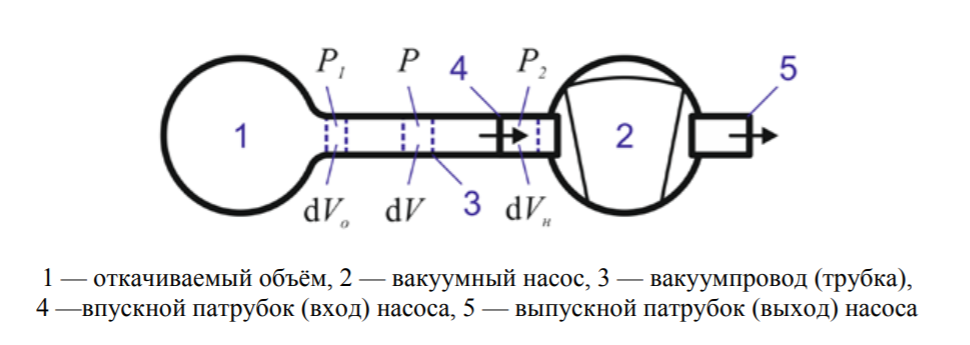
\includegraphics[width = 11 cm]{res/1}
		\caption{Простейшая вакуумная система}
		\label{fig:vac}
	\end{figure}
	
	Быстрота откачивающего действия (скорость откачки) вакуумной системы $S$ -- объем газа, проходящий через рассматриваемое сечение вакуумпровода в единицу времени при текущем давлении
	в данном сечении:
	
	\begin{equation}
		S = \frac{dV}{dT}
	\end{equation}
	
	Следовательно, быстродействие насоса $S_{\text{н}}$ определяется как:
	
	\begin{equation}
		S_{\text{н}} = \frac{dV_{\text{н}}}{dT}
	\end{equation}
	
	а эффективная скорость откачки камеры $S_{\text{o}}$:
	
	\begin{equation}
		S_{\text{o}} = \frac{dV_{\text{o}}}{dT}
	\end{equation}
	
	Падение давления вдоль вакуумпровода $\Delta P = P_1 - P_2$ определяется его пропускной способностью (проводимостью) $U$:
	
	\begin{equation}
		U = \frac{Q}{P_1 - P_2}
	\end{equation}
	где $Q$ -- поток газа через вакуумпровод с соответствующими
	давлениями на концах.
	
	Величина $Z$, обратная проводимости, называется импедансом вакуумпровода:
	
	\begin{equation}
		Z = \frac{1}{U}
	\end{equation}
	
	В общем случае указанные величины $S, U, Q, Z$ как и сами давления $P_1$ и $P_2$ зависят от времени. Но в конце процесса откачки устанавливается квазистационарный режим, при котором поток газа становится практически постоянным и равным количеству поступающего в систему газа
	в единицу времени вследствие наличия течей, т.е. нарушения герметичности (в основном в местах механического соединения отдельных узлов
	вакуумной системы). Для стационарного режима можно записать условие
	непрерывности потока откачиваемого газа:
	
	\begin{equation}
		P_1S_{\text{o}} = PS = P_2S_{\text{н}} = Q
	\end{equation}
	
	Из предыдущих уравнений легко получить, что
	
	\begin{equation}
		\frac{1}{S_{\text{o}}} = \frac{1}{S_{\text{н}}} + \frac{1}{U}
	\end{equation}
	
	Это уравнение позволяет правильно ориентироваться в выборе средств
	откачки и вакуумпроводов при конструировании вакуумной системы для
	любых целей.
	
	Количественной характеристикой течи, является натекание $Q_{\text{н}}$, измеряемое при отключенных средствах откачки:
	
	\begin{equation}
		Q_{\text{н}} = V \frac{P_{\text{к}} - P_{\text{н}}}{\Delta t}
	\end{equation}
	где $V$ -- замкнутый исследуемый объём; $P_{\text{н}}$, $P_{\text{к}}$ -- начальное и конечное давление в объеме; $\Delta t$ -- время между измерениями давления. При наличии течей, нормальной работе средств откачки и отсутствии в системе
	источников паров или газов, зависимость потока газа через течь от времени $Q_{\text{н}}(t)$ носит, как правило, линейный характер.
	
	Для заданного давления $P_1$ в замкнутом исследуемом объёме допустимым считается натекание:
	
	\begin{equation}
		Q_{\text{н}} \ll Q = P_1 S_{\text{o}} = P_1 \frac{S_{\text{н}} U}{S_{\text{н}} + U}
	\end{equation}
	
	На пропускную способность вакуумпровода существенно влияет
	режим течения газа, который характеризуется числом Кнудсена, равным
	отношению длины свободного пробега молекул в газе к характерному
	линейному размеру течения:
	
	\begin{equation}
		Kn = \frac{\lambda}{d}
	\end{equation}
	
	Данная величина характеризует степень разреженности газового
	потока:
	\begin{enumerate}
		
		\item В гидродинамическом (вязкостном) режиме течения ($Kn \ll 1$)
		различают ламинарные и турбулентные потоки. При ламинарном
		течении молекулы газа движутся по параллельным траекториям
		со скоростями, мало отличающимися друг от друга. При турбулентном течении наряду с поступательным движением всей массы газа, молекулы движутся хаотически со скоростями, подвергающимися случайным изменениям
		
		\item В молекулярном (кнудсеновском) режиме ($Kn \gg 1$) течение газа
		сводится к независимому движению отдельных молекул по прямым линиям в периоды между соударениями главным образом со
		стенками вакуумпровода.
		
		\item В переходном режиме ($Kn \thicksim 1$) в системе могут существовать все
		описанные выше виды течения.
		
	\end{enumerate}
	
	В разных режимах течения пропускная способность вакуумпровода имеет существенно различные зависимости от размера его поперечного сечения.
	
	Положим, что за промежуток времени $dt$ давление
	в откачиваемом объёме $V_{\text{o}}$ снижается на $dP_1$. Тогда за промежуток времени $dt$ количество газа поступающего в трубку равно $S_{\text{o}} P_1 dt$, а эта же
	убыль газа в объеме равна $V_{\text{o}} dP_1$, следовательно:
	
	\begin{equation}
		dt = - \frac{V_{\text{o}} dP_1}{S_{\text{o}}P_1}
	\end{equation}
	
	В случае $S_{\text{o}} = const$ иммем 
	
	\begin{equation}
		P(t) = P_1 \exp \left( - \frac{S_{\text{o}}}{V_{\text{o}}}t \right)
	\end{equation}
	
	
	\subsection*{Экспериментальная установка}
	
	Экспериментальный стенд выполнен на основе компактного безмасляного высоковакуумного откачного поста Pfeiffer Vacuum серии HiCube 80 Eco с диафрагменным и турбомолекулярным насосами, вакуумметров Pfeiffer Vacuum серии DigiLine, и вакуумных быстроразъёмных компонентов. Управление основными функциями откачного
	поста, контроль и запись параметров установки осуществляется блоком управления (БУ) через цифровой интерфейс RS-485 с помощью специального программного обеспечения PV TurboViewer.
	
	
	\begin{figure}[H]
		\centering
		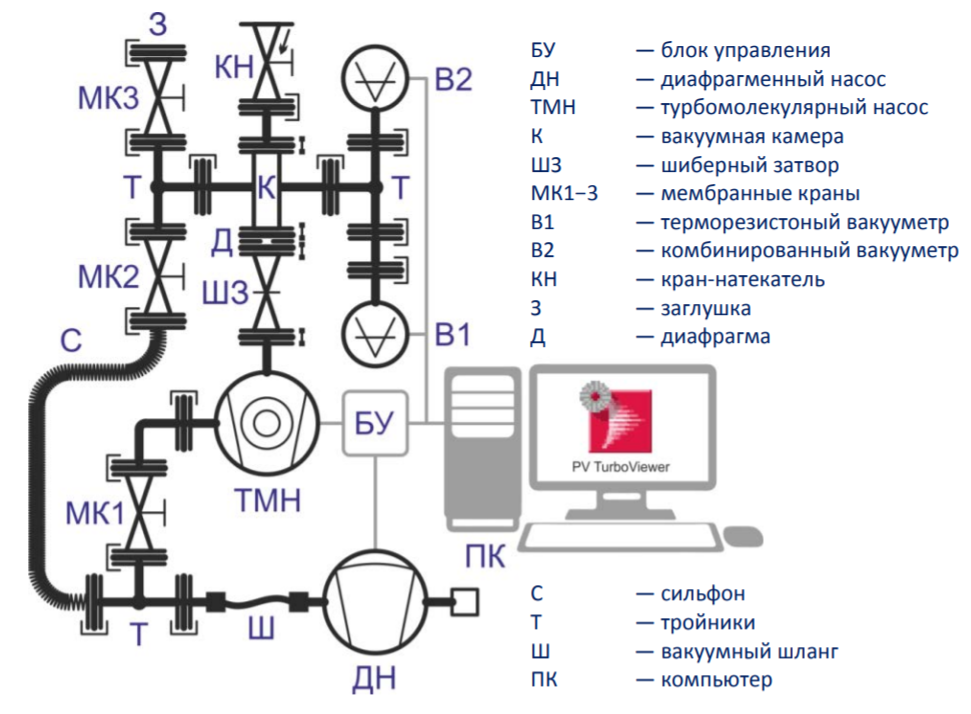
\includegraphics[width = 11.5 cm]{res/scheme.png}
		\caption{Схема экспериментального стенда}
		\label{fig:vac}
	\end{figure}
	\begin{figure}[H]
		\centering
		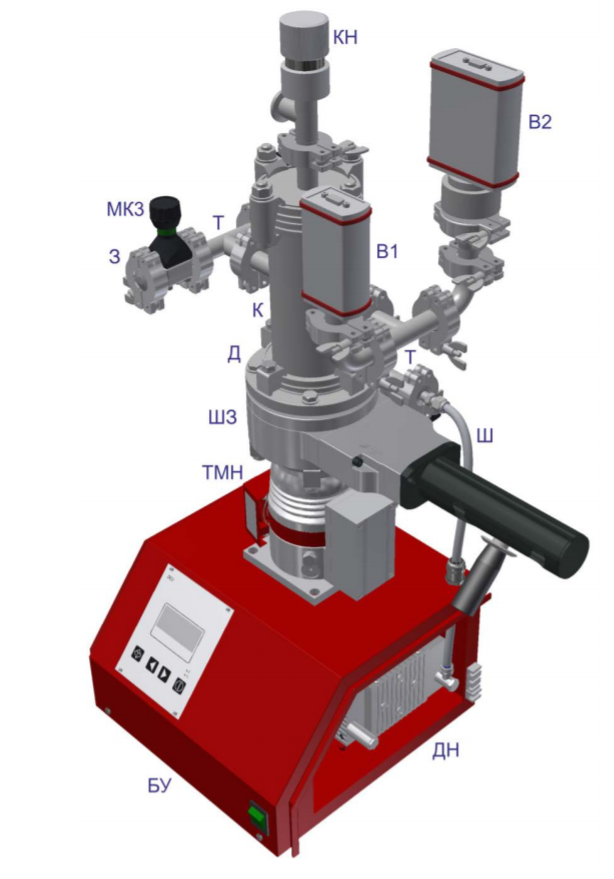
\includegraphics[width = 6.5 cm]{res/picture.png}
		\caption{Внешний вид экспериментального стенда}
		\label{fig:vac}
	\end{figure}
	
	\begin{figure}[H]
		\caption{Технические характеристики вакууметра В1}
		\label{fig:B1}
		\centering
		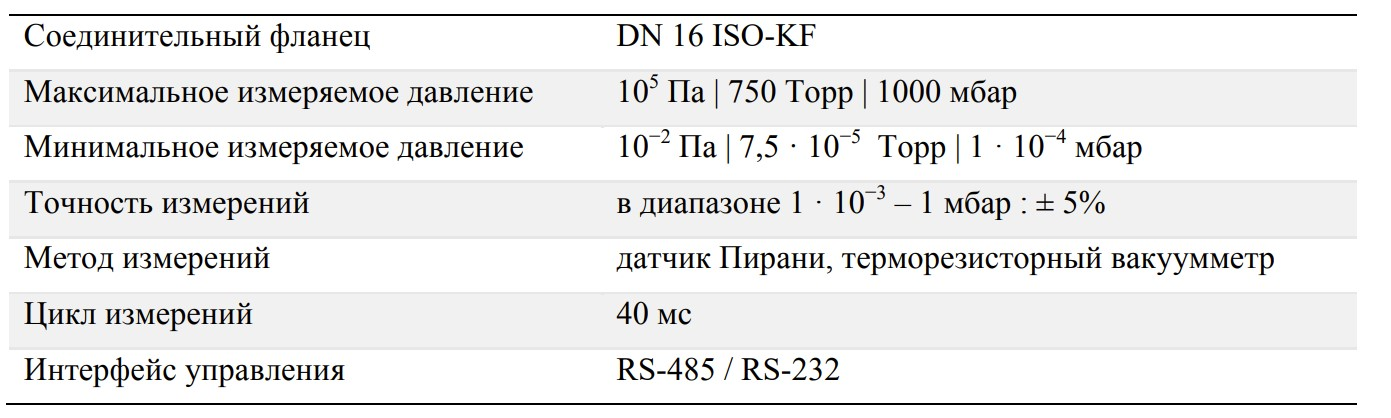
\includegraphics[width = 12 cm]{res/V1_technical.jpg}
	\end{figure}
	\begin{figure}[H]
		\caption{Технические характеристики вакууметра В2}
		\label{fig:B2}
		\centering
		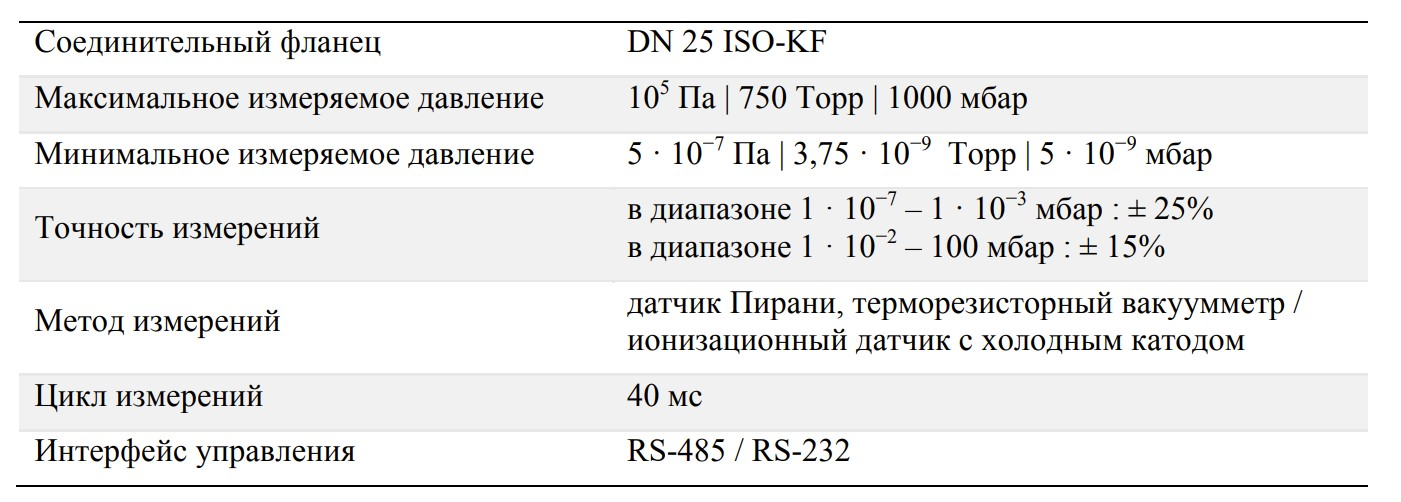
\includegraphics[width = 12 cm]{res/V2_technical.jpg}
	\end{figure}
	
	\section*{Ход работы}
	
	\subsubsection*{Определение объемов частей установки}
	Присоединяя часть известного объёма к установке, можно измерить давление до и после, из закона Бойля-Мариотта получить сам объём кранов установки.
	
	Для этого проделаем следующее:
	\begin{enumerate}
		\item Откачаем установку форвакуумным насосом ДН.
		\item Присоединим к установке сильфон с воздухом при атмосферном давлении.
		\item Выравним давления в сильфоне С и вакуумной камере К экспериментального стенда.
		\item Выравним давление вакуумной камеры К и форвакуумной магистрали установки.
		\item Выравним давление во всей установке, включая объем турбомолекулярного насоса ТМН.
		\item Зафиксируем установившиеся показания вакуумметров.
		
	\end{enumerate}
	
	На каждом этапе выравнивания давления фиксируем его. Было проведено 2 измерения, результаты которых занесены в таблицу \ref{tab:press}.
	
	Погрешности определим, используя технические характеристики вакууметра В2 (см. таблицу \ref{fig:B2})
	
	\begin{table}[h]
		\caption{Результаты измерения давления при различных конфигурациях системы}
		\label{tab:press}
		\begin{center}
			\begin{tabular}{lccc}
				\toprule
				{ } & 1 & 2 & 3 \\ 
				\midrule
				Действие & $p$, мбар & $p$, мбар  & $p$, мбар  \\ 
				\midrule
				Откачка ДН           & 3.8            & 3.6      & 3.6         	   \\ 
				Открытие МК3         & 220            & 190      & 190            \\ 
				Открытие МК2         & 190            & 180      & 180            \\ 
				Открытие МК1         & 140            & 130      & 130           \\ 
				% ^^^^^^^^^^^^^^^^^^^^^^^^^^^^^^^^^^^^^^^^^^^^^^^^^^^^^^^^^
				\bottomrule
			\end{tabular}
		\end{center}
	\end{table}
	
	Объем сильфона $V = 265$ мл.
	% ^^^^^^^^^^^^^^^^^^^^^^^^^^^^^^^^^^^^^^^^^^^^^^^^^^^^^^^^^
	
	Откуда получаем для объемов следующие значения (см. таблицу \ref{tab:volumes}).
	\begin{table}[H]
		\caption{Объемы частей установки}
		\label{tab:volumes}
		\begin{center}
			\begin{tabular}{lc}
				\toprule
				Объем & $(V \pm \sigma_V)$, мл\\ \midrule
				Сильфон                  & $  265 \pm  13$ \\
				Установка                & $ 1771 \pm  89$ \\
				Камера                   & $ 1080 \pm  54$ \\
				Форвакуумная магистраль  & $  125 \pm  47$ \\
				% ^^^^^^^^^^^^^^^^^^^^^^^^^^^^^^^^^^^^^^^^^^^^^^^^^^^^^^^^^
				\bottomrule
			\end{tabular}
		\end{center}
	\end{table}
	
	
	
	Теперь проделаем следующее:
	
	\begin{enumerate}
		\item Отсоединим сильфон от установки.
		\item Откачаем установку форвакуумным насосом ДН.
		\item Откачаем объём турбомолекулярным насосом ТМН.
		\item Видно, что терморезисторный вакуумметр $В1$ достиг своего предела измерений, в то время как комбинированный вакуумметр $В2$ (точнее его магнетронная часть) продолжает отображать корректное давление в системе. Зафиксируем предельное давление в высоковакуумной части установки и время откачки установки насосом ТМН.
		\item Определим уровень течей и скорость откачки системы. Для этого закроем шибер ШЗ, при этом давление в системе начнёт повышаться за счёт наличия течей. Получим таким образом зависимость показаний вакууметра $В2$ от времени. Когда давление превысит $3 \cdot 10^{-3}$ мбар,
		снова откроем шибер. Получим зависимость показаний вакуумметра $В2$ от времени после открытия шибера. Снова зафиксируем предельное давление.
	\end{enumerate}
	
	\subsubsection*{Оценка эффективной скорость откачки системы форвакуумным насосом (ДН)}
	Мы получили зависимость $p(t)$ при откачке системы ДН. Графики этих зависимостей для разных вакууметров приведены на рисунке \ref{fig:p(t)}. Из графика можно сделать вывод, что для определения постоянной времени откачки следует брать показания вакууметра В1. Строим график $\ln{p}(t)$ (см. рис. \ref{fig:lnB1(t)}) и находим параметры полученной кривой \textbf{методом наименьших квадратов}. Вся статистическая обработка занесена в таблицу \ref{tab:lnB1(t)_stat}.
	
	
	\begin{figure}[h]
		\centering
		\includegraphics[width = \linewidth]{res/p(t).pdf}
		\caption{График зависимости $p(t)$ ДН}
		\label{fig:p(t)}
	\end{figure}
	
	\begin{figure}[H]
		\centering
		\includegraphics[width = \linewidth]{res/lnB1(t).pdf}
		\caption{График зависимости $\ln{p}(t)$ ДН вакууметра В1}
		\label{fig:lnB1(t)}
	\end{figure}
	\begin{table}[H]
		
		\caption{Обработка для $Q(P)$}
		\label{tab:lnB1(t)_stat}
		\centering
		\footnotesize
		\begin{tabular}{cc}
			\toprule
			$a \pm \sigma_a$ & $b \pm \sigma_b$ \\
			\midrule
			%
			$-0.0645 \pm 0.0027$     &    $6.344 \pm 4.733$ \\
			$-0.0584 \pm 0.0026$     &    $5.784 \pm 4.547$ \\
			$-0.0587 \pm 0.0028$     &    $5.838 \pm 4.925$ \\
			% ^^^^^^^^^^^^^^^^^^^^^^^^^^^^^^^^^^^^^^^^^^^^^^^^^^^^^^^^^
			\bottomrule
		\end{tabular}
	\end{table}
	
	Систематическую погрешность оценим, как разность коэффициентов наклона графиков. Полную погрешность - как квадратичную сумму случайной и систематической:
	$$S_0 = -a V_0 = (0.26 \pm 0.02) \frac{\text{м}^3}{\text{ч}}$$
	% ^^^^^^^^^^^^^^^^^^^^^^^^^^^^^^^^^^^^^^^^^^^^^^^^^^^^^^^^^
	
	\subsubsection*{Оценка эффективной скорости откачки системы турбомолекулярным (ТМН) насосом}
	Аналогичное рассмотрения зависимости $p(t)$ при откачке системы ТМН, а также статистическая обработка результатов приведена на графике \ref{fig:TMHlnB2(t)} и в таблице \ref{tab:TMHlnB2(t)}. 
	
	\begin{figure}[H]
		\caption{График зависимости $\ln{p}(t)$ ТМН вакууметра В2}
		\label{fig:TMHlnB2(t)}
		\centering
		\includegraphics[width = \linewidth]{res/TMHlnB2(t).pdf}
	\end{figure}
	\begin{table}[H]	
		\caption{Обработка для $Q(P)$}
		\label{tab:TMHlnB2(t)}
		\centering
		\footnotesize
		\begin{tabular}{cc}
			\toprule
			$a \pm \sigma_a$ & $b \pm \sigma_b$ \\
			\midrule
			%
			$-0.0078 \pm 0.0004$     &    $-10.4 \pm 0.6$ \\
			$-0.0072 \pm 0.0008$     &    $-11.2 \pm 2.7$ \\
			$-0.0080 \pm 0.0008$     &    $-11.3 \pm 2.8$ \\
			% ^^^^^^^^^^^^^^^^^^^^^^^^^^^^^^^^^^^^^^^^^^^^^^^^^^^^^^^^^
			\bottomrule
		\end{tabular}
	\end{table}
	
	Аналогично систематическую погрешность оценим, как разность коэффициентов наклона графиков. Полную погрешность - как квадратичную сумму случайной и систематической:
	$$S = aV = 8.3 \pm 0.9 \; \text{мл}/\text{с}$$
	% ^^^^^^^^^^^^^^^^^^^^^^^^^^^^^^^^^^^^^^^^^^^^^^^^^^^^^^^^^
	
	\subsubsection*{Определение уровня течей по ухудшению вакуума после перекрытия откачки насосом ТМН}
	График зависимости $Q_{\text{н}}(t)$ приведен на рисунке \ref{fig:Q(t)}. 
	\begin{figure}[H]
		\caption{График зависимости $Q_{\text{н}}(t)$ вакууметра В1}
		\label{fig:Q(t)}
		\centering
		\includegraphics[width = \linewidth]{res/Q(t).pdf}
	\end{figure}
	
	Для численной оценки натекания построим график $p(t)$ после перекрытия откачки насосом ТМН.
	По угловому коэффициенту определим натекание. Вся статистическая обработка занесена в таблицу \ref{tab:natek}.
	
	\begin{figure}[H]
		\caption{График зависимости $P(t)$ вакууметра В1 после перекрытия откачки насосом ТМН}
		\label{fig:natek}
		\centering
		\includegraphics[width = \linewidth]{res/leaks.pdf}
	\end{figure}
	
	\begin{table}[H]	
		\caption{Обработка зависимости $P(t)$ вакууметра В1 после перекрытия откачки насосом ТМН}
		\label{tab:natek}
		\centering
		\footnotesize
		\begin{tabular}{cc}
			\toprule
			$a \pm \sigma_a$ & $b \pm \sigma_b$ \\
			\midrule
			%
			$2.67e-05 \pm 5.19e-07$     &    $2.69e-04 \pm 1.07e-03$ \\
			$2.06e-05 \pm 3.51e-07$     &    $1.16e-04 \pm 1.38e-03$ \\
			$2.10e-05 \pm 4.18e-07$     &    $1.47e-04 \pm 1.35e-03$ \\
			% ^^^^^^^^^^^^^^^^^^^^^^^^^^^^^^^^^^^^^^^^^^^^^^^^^^^^^^^^^
			\bottomrule
		\end{tabular}
	\end{table}
	
	Откуда получаем оценку натекания: 
	$$Q_{\text{н}} = (0.025 \pm 0.003) \; \frac{\text{мл}\cdot\text{мбар}}{\text{с}}$$
	% ^^^^^^^^^^^^^^^^^^^^^^^^^^^^^^^^^^^^^^^^^^^^^^^^^^^^^^^^^
	
	\section*{Вывод}
	
	По результатам данной лабораторной работы получены следующие результаты:
	
	Значение эффективной скорости откачки форвакуумного насоса по порядку величины сходится с заявленным в характеристиках прибора:
	$$S_0 = (0.26 \pm 0.02) \; \frac{\text{м}^3}{\text{ч}}$$
	$$S_{0(\text{заявл})} = 0.5 \; \frac{\text{м}^3}{\text{ч}}$$
	
	Также получено значение эффективной скорости откачки ТМН:
	$$S = aV = 8.3 \pm 0.9 \; \text{мл}/\text{с}$$
	
	Оценено значение естественной течи:
	$$Q_{\text{н}} = (0.025 \pm 0.003) \; \frac{\text{мл}\cdot\text{мбар}}{\text{с}}$$
	
	$$P S \approx 1.5 \; \text{мбар} \cdot 8.3 \; \text{мл}/\text{с} = 12.4 \; \frac{\text{мл}\cdot\text{мбар}}{\text{с}}$$
	
	Из результатов видно, что:
	$$ Q_{\text{н}} \ll PS $$
	
\end{document}